\section{Introduction {\color{blue} EDITABLE}}\label{sec:intro}

%****NOTES START HERE****


%BRAINSTORMING
%\begin{itemize}
%\item Complexity need not be hard to predict (can %point at the simple predictions paper) [[move to %introduction]]
%\item random walk for example is best predicted by %guess what just happend[[move to introduction]]
%\item The kind of complexity present matters, i.e., %that is whether the complexity is structured or not.%[[use here and mention in intro]]






%\item \col brings about the point nicely that some %prediction strategies cannot utilize the processes internal information transfer method. That is a nonlinear internal information transfer system cannot be predicted effectively with a linear strategy. This gives a practitioner leverage on when to give up and when to keep working. [[use in this section as bridge to next section]]

%\end{itemize}



%\begin{it}
%Paragraph on computer performance, including citations to Todd paper
%and summary of the results that indicate that they're deterministic
%nonlinear dynamical systems.  Given that, we should be able to
%predict.  What benefits would accrue if we could do so: power mgmt,
%end world hunger [[this is my primary goal everyday :)]], etc.
%\end{it}
%Things to add to introduction
%\begin{enumerate}

%\item \cmark Make an argument that Computer Performance %is a great testing ground as it gives signals that completely cover the spectrum of complexity \col \dots \gcc

%\item When deterministic structure even complex structure exists that structure can be utilized for prediction.
%\item For noisy real-valued time series distinguishing randomness (WN,RW) complexity from structured nonlinear / chaotic /high period / high dimensional etc complexity is (until now) very hard.
%\subitem for this provide predictions of \gcc and \col side by side and discuss "How can we tell if we did a bad job because the method is inadequate vs the signal being too complex. Lead this into is it possible to tell if there exists structure in a time series to know if we should find a better model or not. Maybe even having 4 predictions. top being ARIMA of the above signals and bottom being LMA of the above signals. Show that one improved and one did not. Is it that we used the wrong method to predict or is it that we simply can't predict the signal better than a random walk due to high levels of internal signal complexity.



%\item\cmark Introduce the two main contributions of the paper which are outlined at the begining of the results section

%\end{enumerate}
%\noindent ***NOTES END HERE****
%
%\noindent ****SECTION START****


Complicated time series are ubiquitous in modern scientific research.
Every observed time series, complicated or not, exists on a spectrum of \emph{complexity}. On the low end of that spectrum are time series that exhibit perfect predictive structure, i.e, signals whose future value are perfectly predicted by knowledge of past values from some ``ideal" model. In particular, there is a an underlying process that generates and transmits information from the past to the future in a perfectly predictable fashion. Some examples of this are constant or low-period signals. On the opposite end of this spectrum are signals which are ``fully complex", i.e., the underlying generating process creates information so rapidly that no information at all is transmitted from the past to the future. Some examples, of this are white noise or random walk processes. With signals on this side of the spectrum, knowledge of the past gives absolutely no insight into the future, \emph{regardless} of the chosen model.  In the middle of this spectrum are where complicated \emph{and} interesting---from a modeling perspective---signals exist, e.g., observations of a deterministic chaotic trajectory, high period signals with some level of noise on top, etc. With time series in this portion of the spectrum, enough information is being transmitted from the past to the future that given the \emph{ideal} model the future of the observed system could be forecast with high accuracy.

Unfortunately, as a corollary of the undecidability of the halting problem: there cannot exist \emph{one} universally ideal forecasting scheme for even completely noise-free deterministic time series\cite{weigend-book}, let alone an arbitrary time series. This naturally leads to an important and hard question: given a complicated real-valued time series, does their exist a forecast model for that time series that can utilize the information being transmitted from past to future (if such information exists)? A first step in answering this question is to answer: is it possible to reliably quantify where on the spectrum of complexity the time series lies? i.e, when little or nothing is known about the underlying system's generating process (e.g., linear, nonlinear, deterministic, stochastic, stationary, non-stationary etc.) can it be inferred without a model if the signal is too \emph{complex} to effectively forecast? Since the information in an observation can be partitioned into two pieces --- redundancy and entropy generation\cite{crutchfield2003} --- our goal is to analyze how the amount of predictive structure present in a signal, as measured by the redundancy, relates to the performance of prediction strategies. The formation of this spectrum or partition as well as what is meant by \emph{low, medium and high} complexity are visited in more detail in Section \ref{sec:meaComplex}.


To answer this question and for the purposes of this paper we focus on real-valued (possibly) noisy scalar time series which appear \emph{complicated}, i.e., they exhibit interesting behavior, for instance, not of low period, strictly monotonic, or constant. We make no assumptions about the generating process's properties,(e.g., linear, nonlinear, deterministic, stochastic, stationary, non-stationary, etc.) and we attempt to measure empirically where on the previously mentioned spectrum of \emph{complexity} the time series exists.
We argue that an extension of \emph{permutation entropy}
\cite{bandt2002per}---a method for approximating the entropy of a real-valued-finite-length-noisy time series through ordinal analysis---is an effective way to explore that conjecture. In light of this, for the purposes of this paper we define \emph{complexity} as a particular approximation of Kolmogorov-Sinai \emph{entropy}[[Probably need a citaiton for KS entropy]], which we define and explain rigorously in Section \ref{sec:meaComplex}. In this fashion a random walk time series (which exhibits high entropy) is purely complex, where as a periodic signal (which exhibits low entorpy) has low complexity. The permutation entropy is ideal in a situation like this as it converges on the true entropy value, unlike other partitioning techniques used in the past which either require specific knowledge of the generating process or produce biased values of the entropy~\cite{bollt2001}.


%[[Introduce and make it clear why we choose comp. perf. as test bed.]]

To explore this conjecture we require a test bed for generating a broad array of time series which cover the full spectrum of complexity. We argue that the ideal test bed for this purpose are computer performance traces, e.g., the processor efficiency during the execution of a particular program. Computers are among the most complex engineered artifacts in current
use.  Modern microprocessor chips contain multiple processing units
and multi-layer memories, for instance, and they use complicated
hardware/software strategies to move data and threads of computation
across those resources.  These features---along with all the others
that go into the design of these chips---make the patterns of their
processor efficiency highly complicated.
%Accurate forecasts of these quantities, if one could
%construct them, could be used to improve computer design.
% If one
%could predict that a particular computational thread %would be bogged
%down for the next 0.6 seconds waiting for data from main memory, for
%instance, one could save power by putting that thread %on hold for that
%time period (e.g., by migrating it to a processing %unit whose clock
%speed is scaled back).

As a result computer performance traces are very
complicated and range across the entire spectrum of complexity, making this an ideal test bed.  Even a simple ``microkernel," like a three-line loop that
repeatedly initializes the upper triangle of a matrix in column-major order, can produce everything from periodic to
chaotic performance traces \cite{mytkowicz09}, depending on the architecture running the software. Such a performance trace is shown in
Figure~\ref{fig:ipc}.%, and chaos places fundamental limits on predictability.
%
 \begin{figure}[htbp]
    \centering
    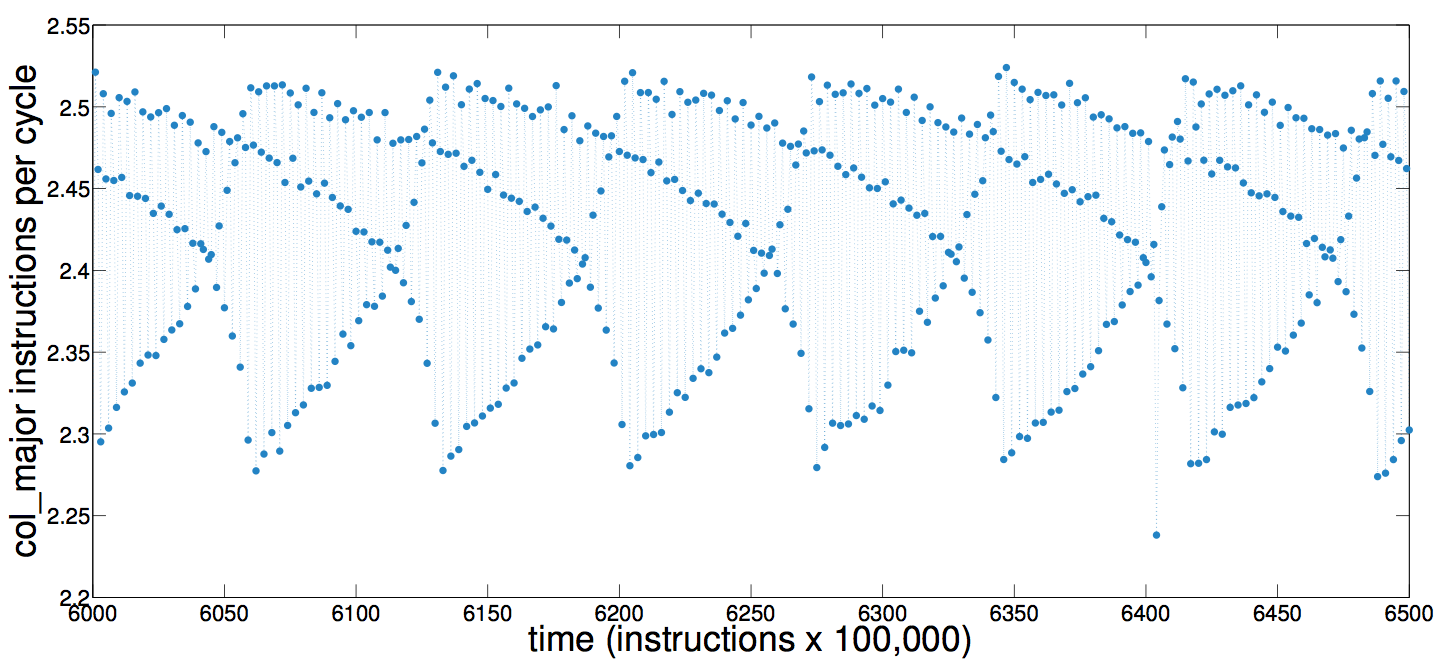
\includegraphics[width=\textwidth]{figs/colshortts}
    % where an .eps filename suffix will be assumed under latex,
    % and a .pdf suffix will be assumed for pdflatex
    \caption{A small snippet of the instructions per cycle(ipc) of \col, a three-line C program that repeatedly initializes
      a matrix in column-major order, running on an Intel i7\textsuperscript{\textregistered}-based machine.}
   \label{fig:ipc}
  \end{figure}
%
More interesting programs, e.g., compilers and numerical solvers, produce time series which exist throughout the spectrum of complexity: from completely predictable to completely unstructured,i.e., low to high complexity[[Just trying to reinforce the wording in the readers mind]]. In addition, some performance traces even exhibit interesting regime changes as a program switches between varying subroutines. With a single system (computer performance) capable of producing complicated time series that vary so greatly in complexity (periodic to noise), it would be invaluable to known a priori if a trace contained enough predictive structure to build a  forecast model based on structure before time and effort was spent searching for an ideal model.

%The computer systems community has applied a variety of prediction
%strategies to traces like this, most of which employ regression.  An
%appealing alternative builds on the recently established fact that
%computers can be effectively modeled as deterministic nonlinear
%dynamical systems \cite{mytkowicz09}.  This result %implies the
%existence of a deterministic forecast rule for those %dynamics.  In
%particular, one can use \emph{delay-coordinate %embedding} to
%reconstruct the underlying dynamics of computer %performance, then use
%the resulting model to forecast the future values of computer
%performance metrics such as memory or processor loads
%\cite{josh-ida2011}.  In the case of simple microkernels like the one
%that produced the trace in Figure~\ref{fig:ipc}, this deterministic
%modeling and forecast strategy works very well.  In more-complicated
%programs, however, such as numerical software or compilers,
%this forecast strategy---as well as the traditional methods---break
%down some of the time, but work fine others.








This paper provides insight into when, why, and how forecast strategies fail when they are applied to complicated time series by empirically estimating their inherent complexity. [[Liz, do you think here would be better for the sentence about we are not the first, or is above where I asked Ryan to insert it ok? I worry it would muddy the water of this synopsis paragraph.]] We focus here on the specific example of
computer performance but believe the results apply to a much broader class of time series. We conjecture that the complexity of traces
from these systems---which results from the inherent dimension,
non-linearity, and non-stationarity, as well as from
measurement issues like noise, aggregation, and finite data
length---is \emph{empirically quantifiable}. To validate this conjecture we model 120 different performance traces using a variety of forecasting models which we introduce in Section \ref{sec:model}. We then compare the empirically estimated \emph{complexity} with the accuracy of each forecast method. Which results in two primary findings:


\begin{enumerate}

\item The complexity of a noisy real-valued time series is quantifiable and correlated with prediction accuracy of an ideal predictor.

\item The way information is processed internally by a given process plays a crucial role in the success of different forecasting schema.

\end{enumerate}


%We argue that \emph{permutation entropy}
%\cite{bandt2002per}, a method for measuring the %entropy of a
%real-valued-finite-length time series through ordinal %analysis, is an
%effective way to explore that conjecture.  %{\color{red} Probably remove this and move a%s it is in the experimental methods or point to that section for more details}We study three
%examples---a simple microkernel and two complex %programs: one from the
%SPEC 2006CPU benchmark suite, and one from LAPACK---%running on an Intel i7-based machine.  For
%each program, we calculate the permutation entropy of %the processor
%load (instructions per cycle), then compare that to %the prediction accuracy attainable for
%that trace using a series of deterministic models.

% paragraph to appease the theoretician in me
It is worth taking a moment to consider the theoretical possibility of
this task. We are not attempting to predict the state of the CPU at an
arbitrary point in the future --- this, at least with perfect
accuracy, would be tantamount to solving the halting problem. What we
are attempting is to predict aspects or functions of the running of
the CPU, e.g., processor efficiency and similar statistics. Prediction of these quantities
at some finite time in the future, even with perfect accuracy, does
not violate the Rice-Shapiro theorem~\cite{hopcroft} which essentially states that any non-trivial property of a program is uncomputable.

 The rest of the paper is organized as follows: Section~\ref{sec:related} discusses similar methods and how this method is different. Section~\ref{sec:methods} explains the experimental setup and explains in depth the programs observed to generate each time series. Section~\ref{sec:model} describes the four forecast models we implemented.  In
 Section~\ref{sec:meaComplex}, we review weighted permutation entropy. In Section~\ref{sec:results} we estimate the complexity of each time series, and
 compare the complexity to the prediction accuracy of several different forecast schema.  In
 Section~\ref{sec:conc}, we discuss these results and their
 implications in regard to our conjecture, and consider future areas of
 research.

